\chapter{Avanced orientation}



%=======================================================================================================
\section{Creating a calibration unknown by images}

  % - - - - - - - - - - - - - - - - - - - - -
\subsection{When is it necessary ?}

It sometimes happens that each image, or each group of images,
has been acquired with a different set of internal parameters. Here
are possible case :

\begin{itemize}
    \item when the images were acquired with autofocus, which create variation
          of the focal length (in macro photo, the focal length when focus is
          at $\infty$ is half the focal length when the focus is at image ratio of $1:1$),


    \item when  the image stabibilizer is free, this create (at least)
          variation of principal point;

    \item when  image where acquired with variable  zooming .
\end{itemize}


From a photogrammetric point of view, these case must be avoided
as much as possible; however there are case where the user has no
choice.

  % - - - - - - - - - - - - - - - - - - - - -
\subsection{Examples}

The directory {\tt applis/XML-Pattron/Oiseau-Margot/} contains XML
files that where used to process images acquired with macro lenses.
The files {\tt New-Apero1.xml} to {\tt New-Apero6-ExportDirPlanMM.xml}
contains example on real case of the different mechanisms exposed
here. By the way, these example may be a bit complex because they
were made before key standardisation.

See especially the examples {\tt Apero-ExCalibPerIm-1.xml} and
{\tt Apero-ExCalibPerIm-2.xml} on {\tt MurSaintMartin}, that have
been added after writing this section; they are more realistic
and contain some comments at the begining that should be
sufficient.

  % - - - - - - - - - - - - - - - - - - - - -
\subsection{How to create unknowns}

The optional section {\tt <CalibPerPose>}, under {\tt <CalibrationCameraInc>},
allow to handle these cases. It contains a mandatory args {\tt   <KeyPose2Cal>}:


\begin{itemize}
    \item it must constain a string $K$ which describe  a key association,
          (see~\ref{Ref:Key:Map}  for {\tt <KeyedNamesAssociations>});
    \item  two images  $I_1$ and $I_2$ will share the same internal parameters,
           if and only if $K(I_1) = K(I_2)$;
     \item for example  if $K$ is the identity key, a new calibration will
           be create for each new image;

     \item  for each of these calibration, the identifier will be $K(I)$ and not,
            as usual, the tag {\tt <Name>}; this is necessary because elsewhere 
             different internal calibration would have the same identifier;

      \item this identifier is used when it is necessary to refer
            to a set of internal calibration (for example when applying
            constraint only to a subset of the existing calibration);

\end{itemize}

  % - - - - - - - - - - - - - - - - - - - - -
\subsection{Saving  results with  variable calibrations}

The most current case for using these mecanisms is when there is one calibration
per image. In this case, the easiest way for handling the results, is  to 
simply  save the internal calibration  with the external calibration;
this is, by default, what Apero does  in {\tt <ExportPose>}, see 
{\tt Apero-0.xml} in~\ref{Result:Apero0}.


For more complicated case,  an {\tt <ExportCalib>} section  will have to be 
used with the following tags :

\begin{itemize}
    \item {\tt <PatternSel>}  to specify to wich calib it applies; the selection
         is made on the identifier (here $K(I)$);

    \item {\tt <KeyAssoc>}  to specify how to compute a file name from the identifier;

    \item {\tt <KeyIsName>}  at {\tt false} \footnote{which is, however, the default value} meaning
          that {\tt <KeyAssoc>}  is a key and not an absolute name;
\end{itemize}


  % - - - - - - - - - - - - - - - - - - - - -
\subsection{Loading initial values  with  variable calibrations}

When  variable internal calibration is used a first time, 
the different calibration can be initialized with the same
value.  This value can be read as usual in the {\tt <NameFile> } of {\tt <CalValueInit>}.
See an example in {\tt  applis/XML-Pattron/Oiseau-Margot/New-Apero1.xml},

There is other cases, where it will be needed to initialize these  calibration
from variable values; for example values  that have been computed and saved by a
previous runing of Apero. In this case, a {\tt KeyedNamesAssociations} will be used 
to specify the association between \emph{the  name of the pose} and file where 
the initial value is to be read; this key is specified in the optional
{\tt <KeyInitFromPose>}; see example in {\tt  applis/XML-Pattron/Oiseau-Margot/New-Apero3.xml}.


\subsection{Examples with group of pose}

Sometime we do not want to create a calibration for each image,
but a calibration for each group of image. This can occurs
when we know that that the parameters influencing the calibration
(zoom, focus) have changed, but only a few time, and we are able
to specify which group of image share the same parameters.
This can occurs also when we have used several version of the
same camera with the same focal lenght (so not distinguable
with the procedure used in Tapas).

See {\tt Apero-ExCalibPerGROUPIM-1.xml} and 
{\tt Apero-ExCalibPerGROUPIM-2.xml}  on  {\tt MurSaintMartin} data
set, it illustrate how this can be done. The file contains
some comments.


The file {\tt Apero-ExCalibPerIm-1.xml} and {\tt Apero-ExCalibPerIm-2.xml}  
on  {\tt MurSaintMartin} have been added and contain also
example for calibration per images that are probably easier to understand
than {\tt  applis/XML-Pattron/Oiseau-Margot/}.

%=======================================================================================================

\section{Data base of existing calibration}

\label{DB:Calib}
\subsection{Generalities}


%=======================================================================================================
\section{Auxilary exports}

  % - - - - - - - - - - - - - - - - - - - - -

\subsection{Generating point clouds with {\tt <ExportNuage>}}

\label{Ap:Exp:Nuage}


%=======================================================================================================

\section{Using scanned Analog images}

\label{Analog:Image}
Scanned analog images, are important in many application because  they are
a valuable source of information for studying phenomens on long periods.
From the photogrammetric point of view, the main difference between 
scanned images and numerical camera is that for each images, there
is a speccific  tranformation between the photo and the scanner.
This tranformation can be computed when there exist fiducial marks 
on the camera. This section study how this can be done in {\tt Apero/MicMac}.


The directory {\tt DemoScanned/} contains a data-set that illustrates the
functionnalities. It contains $5$ images that are a simulation of scanned
iamges : the image have been randomly rotated and scaled, simulating the
interior orientation of the scanner, before the rotation $8$  fiducial marks have
been added. Figure~\ref{ImFid} illusrate this data set.


\begin{figure}
\begin{tabular}{||c|c||}
   \hline \hline
   \multicolumn{2}{c|}{\includegraphics[width=120mm]{FIGS/Niche/ImGlob.jpg}} \\ 
   \includegraphics[width=40mm]{FIGS/Niche/Cible1.jpg} &
   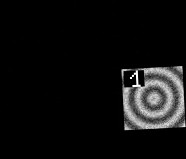
\includegraphics[width=40mm]{FIGS/Niche/Cible2.jpg} 
\end{tabular}
\caption{Simulation of fiducial marks : an image and two marks }
\label{ImFid}
\end{figure}


For process Processing such  data set, compared to "classical" numerical images,
there is two slight differences :

\begin{itemize}
   \item the position of fiducial mark on images and on the camera has to be indicated;
   \item the calibration will not be expressed in pixel, but in the same unit
         that the position of the reference fiducial marks (generally $mm$).
\end{itemize}

On {\tt DemoScanned/}, the directory {\tt Ori-InterneScan/}, contains all the information
about the fiducial marks. It functions this way :

\begin{itemize}
    \item each file contains a structure a type {\tt <MesureAppuiFlottant1Im>} wich describe a list
          of named points (here the names are {\tt P0, P1, \dots}; this is the same structure used
          for image measurement of GCP, as seen in~\ref{GCP:Org};

     \item there is a file {\tt MeasuresCamera.xml} that contains the position of the fiducial marks
          on the camera;
   
     \item for each image {\tt XXX}, there is a file {\tt MeasuresIm-XXX.xml} that contain the position
           of the marks in the image; when this file do not exist, the image is considered to be a "classical"
           numerical image, that will be processed as usual;

     \item if required \footnote{for example if several analog camera are used in the same bundle}
           it is possible to change the association between an image and the two file :position in  camera
           and image; for this change the  value of {\tt Key-Assoc-STD-Orientation-Interne}
           \footnote{see in include/XML\_GEN/DefautChantierDescripteur.xml the default value}
           in your {\tt MicMac-LocalChantierDescripteur.xml}
\end{itemize}

Here, the file {\tt MeasuresCamera.xml} contains the position of fiducial marks in $mm$,
all the calibration  must then given with the same unit and in the same repair that these
marks. For technicall reason, this repair must be the uper left corner and not the center.
As {\tt Apero/MicMac} cannot deal correctly with default calibration in $mm$, we 
have to give an initial value in file {\tt Ori-CalibInit}. Some comments on this file ;

\begin{itemize}
    \item  the sz of image {\tt <SzIm>} is also in $mm$ (as the normalization focale
            {\tt <Etats>}  and all parameters).
     \item  the optional {\tt  <ScannedAnalogik> } is set to true, this is required because
            it will indicate to {\tt Apero} to be "tolerant" is tie points are detected out 
            of the bounding box $[0,0]x[24,36]$;
\end{itemize}

The file {\tt ExCmd.txt} contains a possible processing of the data :


\begin{itemize}
    \item {\tt Tapioca  All ".*jpg"  1200}  , as usual \dots
    \item {\tt Tapas  FishEyeBasic  ".*jpg"  Out=Ori1 InCal=CalibInit PropDiag=0.68}

     \begin{itemize}
          \item  it is necessary to indicate the calibration in {\tt CalibInit} in $mm$ because {\tt Apero}
                 would not built it correctly;
          \item no need to indicate situation of fiducial mark, the def value of {\tt Key-Assoc-STD-Orientation-Interne}
                will make {\tt Apero} look for them at the wright place;
           \item {\tt PropDiag=0.68} , because it is a hemi-spherik fisheye; 
      \end{itemize}

    \item {\tt Tapas FishEyeBasic ".*jpg" InOri=Ori1  Out=Ori2 PropDiag=0.68} 
    \begin{itemize}
           \item  just to check that {\tt Tapas} can be iterated in  this  configuration
    \end{itemize}
    \item {\tt Malt GeomImage ".*jpg" Ori2 Master=IMG\_5693\_Out.jpg Spherik=true SzW=2} 
    \begin{itemize}
             \item the {\tt Spherik=true} is well adapted  to the scene, in this geometry 
                   {\tt MicMac} compute the depth  $R=f(i,j)$ where $R$ is the distance
                   to the master image center \footnote{i.e. rectification is made on sphere};
    \end{itemize}

    \item {\tt Nuage2Ply MM-Malt-Img-IMG\_5693\_Out/NuageImProf\_STD-MALT\_Etape\_8.xml Attr=IMG\_5693\_Out.jpg Scale=2}

    \begin{itemize}
             \item usual generation of point cloud in ply format, figure~\ref{ImNiche} illustrates;
    \end{itemize}

\end{itemize}




\begin{figure}
   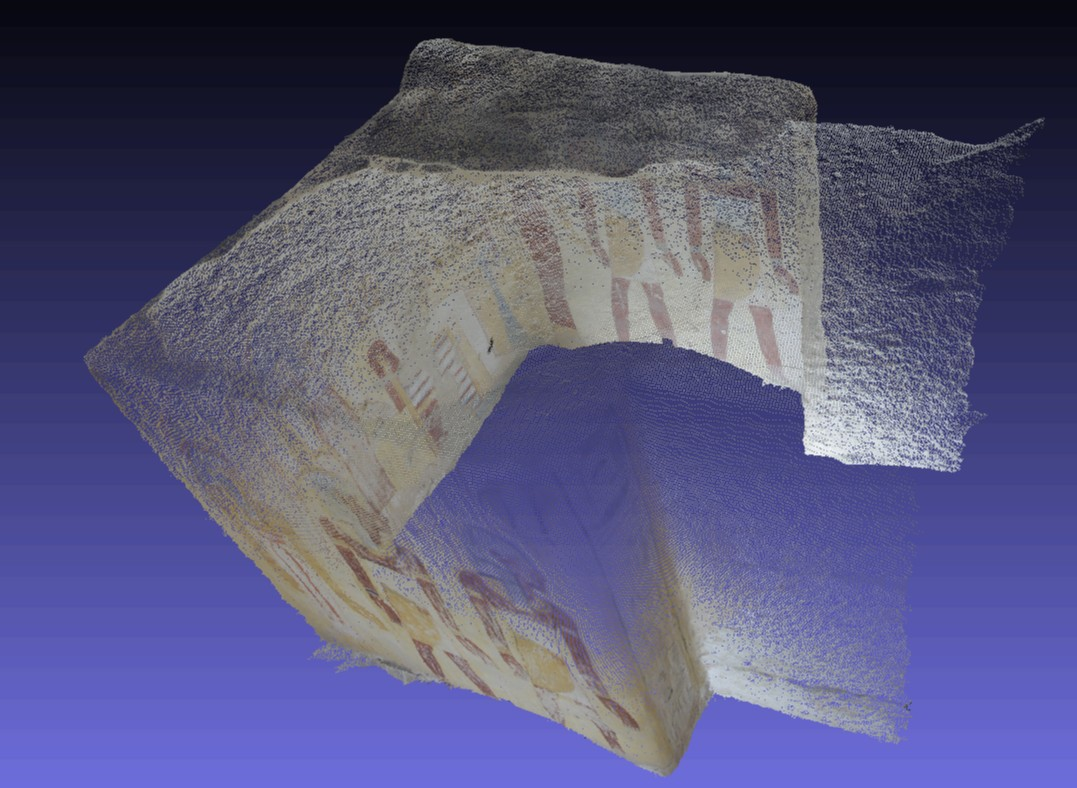
\includegraphics[width=120mm]{FIGS/Niche/snapshot00.jpg} 
\caption{Point cloud with simumlation of scanned images}
\label{ImNiche}
\end{figure}


If you take a look at orientation files, you will see that they are self sufficient for
matching : the {\tt <OrIntImaM2C>}  section contains the affinity from scanner to image computed
from the fiducial marks from scanner to image computed
from the fiducial marks :

\begin{verbatim}
     <OrientationConique>
...
          <OrIntImaM2C>
               <I00>2753.06179948014324 1771.95961861625119</I00>
               <V10>-72.5948450058228758 4.58183503308403939</V10>
               <V01>-4.5818350330840607 -72.5948450058228332</V01>
          </OrIntImaM2C>
...
     </OrientationConique>
\end{verbatim}



